% ============================================================================
% Cross-Attentive Wavelet-Transformer (CAWT) for ECG Arrhythmia Classification
% IEEE Conference Format — Two-Column
% ============================================================================
\documentclass[conference]{IEEEtran}
 
% ---- Packages ----
\usepackage[utf8]{inputenc}
\usepackage[T1]{fontenc}
\usepackage{amsmath,amssymb,amsfonts}
\usepackage{graphicx}
\usepackage{booktabs}
\usepackage{multirow}
\usepackage{array}
\usepackage{hyperref}
\usepackage{cite}
\usepackage{algorithm}
\usepackage{algorithmic}
\usepackage{float}
\usepackage{textcomp}
\usepackage{xcolor}
\usepackage{balance}
\usepackage{subcaption}

\usepackage{tabularx}
\usepackage{tikz}
\usetikzlibrary{arrows.meta, positioning, fit, calc, backgrounds}
 
\graphicspath{{figs/}}
 
\hypersetup{
    colorlinks=true,
    linkcolor=black,
    citecolor=black,
    urlcolor=blue
}
 
% ============================================================================
\begin{document}
 
\title{Cross-Attentive Wavelet-Transformer (CAWT) for ECG Arrhythmia Classification}
 
\author{%
\begin{tabular*}{\textwidth}{@{\extracolsep{\fill}}ccc@{}}
\begin{tabular}[t]{c}
\textbf{M. P S S S Hari Chandra Hlada} \\
\textit{Student, Dept. of ECE} \\
\textit{MVGR College of Engineering (A)} \\
Vizianagaram, India \\
harichandra3001@gmail.com
\end{tabular}
&
\begin{tabular}[t]{c}
\textbf{K. Varshini} \\
\textit{Student, Dept. of ECE} \\
\textit{MVGR College of Engineering (A)} \\
Vizianagaram, India \\
killadavarshini5@gmail.com
\end{tabular}
&
\begin{tabular}[t]{c}
\textbf{L. P. Harshita} \\
\textit{Student, Dept. of ECE} \\
\textit{MVGR College of Engineering (A)} \\
Vizianagaram, India \\
lpharshita.06@gmail.com
\end{tabular}
\\[4em]
\begin{tabular}[t]{c}
\textbf{K. Raj Samuel} \\
\textit{Student, Dept. of ECE} \\
\textit{MVGR College of Engineering (A)} \\
Vizianagaram, India \\
samuelkillo462@gmail.com
\end{tabular}
&
\begin{tabular}[t]{c}
\textbf{Dr. M. Lakshmi Prasanna Rani} \\
\textit{Associate Professor, Dept. of ECE} \\
\textit{MVGR College of Engineering (A)} \\
Vizianagaram, India \\
prassugowtham@gmail.com
\end{tabular}
&
\\
\end{tabular*}
}
 
\maketitle
 
% ============================================================================
% ABSTRACT
% ============================================================================
\begin{abstract}
Classifying heartbeats from single-lead ECG recordings is hard, mostly because abnormal beats are rare and look different from one patient to the next. Existing hybrid CNN-Transformer models typically run the convolutional stage first, then hand off features to a Transformer. This creates a one-way pipeline where the Transformer never gets to tell the CNN what to pay attention to. This paper presents the Cross-Attentive Wavelet-Transformer (CAWT) to address that limitation. CAWT has two parallel branches: one extracts multi-scale frequency features through convolutions at kernel sizes 3, 7, 15, and 31, while the other processes the raw beat as a temporal sequence. Instead of fusing their outputs at the end, the two branches talk to each other at three intermediate depths through bidirectional cross-attention with Rotary Position Embeddings (RoPE). Class imbalance is a serious concern here (fusion beats make up less than 1\% of the MIT-BIH dataset), so it is handled with SMOTE applied after the train/test split, inverse-frequency sample weights, and a focal loss ($\gamma = 2.0$) with label smoothing ($\epsilon = 0.1$). On the MIT-BIH Arrhythmia Database under the five-class AAMI protocol, CAWT reaches 99.00\% accuracy, 93.77\% macro F1, and 0.9883 AUROC. In ablation runs, replacing bidirectional coupling with late fusion dropped accuracy to 96.12\%, confirming that the repeated cross-branch exchange is doing real work.
\end{abstract}
 
\begin{IEEEkeywords}
Arrhythmia detection, bidirectional cross-attention, multi-resolution convolution, Rotary Position Embedding, focal loss, MIT-BIH database.
\end{IEEEkeywords}
 
% ============================================================================
% I. INTRODUCTION
% ============================================================================
\section{Introduction}
 
\IEEEPARstart{C}{ardiac} arrhythmias are responsible for a significant portion of sudden cardiac deaths worldwide. The tricky part is that many arrhythmias, such as supraventricular ectopics or fusion beats, show up intermittently and can go completely unnoticed between episodes~\cite{kreatsoulas2010, joshi2008}. A typical 24-hour Holter recording produces upwards of 100,000 individual heartbeats, and expecting a cardiologist to review all of them manually is unrealistic. Even in controlled lab settings, de Chazal et al.~\cite{dechazal2004} showed that trained annotators end up disagreeing on the same beats. So if the experts themselves cannot get consistent labels, manual screening is not going to scale with the data volumes wearable monitors produce today. That is the motivation behind this work.
 
Before deep learning, the standard approach was to hand-pick features like R-R intervals and QRS widths, then feed them into a classifier. This works for textbook beats but falls apart for anything unusual~\cite{singh2022}. CNNs improved things by learning features (QRS shape, ST-segment deviation) directly from the raw signal~\cite{abdelminaam2022}. Transformers took a different route and used self-attention to capture long-range dependencies across the entire beat sequence~\cite{vaswani2017, kim2025, dhara2025}. Each approach covers what the other misses, which is why people started combining them.
 
Most existing hybrid models do this in a straight line: the CNN processes the signal first, produces features, and passes them to a Transformer. The problem is that the Transformer only reads what the CNN gives it. The CNN has no idea what the Transformer would have found useful. A few papers add cross-attention between the two, but only at the very end~\cite{hu2022, lee2024}, after the CNN has already finished extracting features. Early experiments with a similar sequential setup showed that the CNN consistently misclassified fusion beats (class F) as normal, because it could not see that the Transformer had flagged an unusual R-R interval pattern.
 
CAWT was designed to fix that bottleneck. The input is split into two branches: one processes multi-scale frequency content (kernel sizes 3, 7, 15, 31), the other handles the raw temporal sequence. The two branches exchange information \emph{three times} during feature extraction through bidirectional cross-attention guided by Rotary Position Embeddings (RoPE). This way, the CNN can adjust its filters based on what the Transformer has already spotted, and vice versa.
 
CAWT was tested on the MIT-BIH Arrhythmia Database using the AAMI five-class grouping, and it outperformed both single-branch baselines and the late-fusion alternative. The main contributions of this paper are:
 
\begin{enumerate}
    \item A dual-branch design where parallel convolutions at four kernel scales capture frequency structure while a separate temporal branch models sequential patterns.
    \item A three-stage bidirectional cross-attention bridge with RoPE that lets both branches refine each other during training, not just at the output.
    \item A class-imbalance pipeline (post-split SMOTE, inverse-frequency weighting, focal loss) that pushes fusion-beat recall from near-zero in the WaveletCNN baseline to 88\% in the full model.
    \item Ablation experiments showing where the gains actually come from: late fusion vs.\ unidirectional vs.\ bidirectional coupling, one stage vs.\ three.
\end{enumerate}
 
% ============================================================================
% II. RELATED WORK
% ============================================================================
\section{Related Work}
 
\subsection{Handcrafted Feature Methods}
Earlier work on arrhythmia classification relied heavily on manually designed features. For instance, Ullah et al.~\cite{ullah2024} used Particle Swarm Optimization to select features and ran them through an Extra Trees classifier, which gave decent results on common arrhythmia types. Philip and Hemalatha~\cite{philip2023} found that how the beats are segmented matters more than which classifier is used, which motivated the preprocessing effort in Section~III-B. The downside of these methods is that they only work for beat shapes the features were designed to capture.
 
\subsection{Deep Sequence Models}
End-to-end learning removed the need for manual feature design. Saadatnejad et al.~\cite{saadatnejad2020} combined continuous wavelet features with LSTM networks to build a classifier suited to low-power wearable devices. Cai et al.~\cite{cai2020} developed Multi-ECGNet, a multi-branch CNN framework for simultaneously predicting co-occurring arrhythmia labels. Wei and Li~\cite{wei2025} proposed a multi-scale CNN operating in parallel across several temporal resolutions, whose outputs are then processed by a Transformer encoder. This architecture is closely related to ours but lacks bidirectional coupling between branches.
 
\subsection{Hybrid CNN-Transformer Designs}
Several groups have tried combining CNNs with attention mechanisms. Lee et al.~\cite{lee2024} added cross-stage feature sharing between convolutional and attention modules to cut redundancy. He et al.~\cite{he2025} built CardioAttentionNet, which pairs depthwise convolutions with a BiLSTM and keeps the model small enough for portable devices. A common pattern across all of these papers is that information only flows in one direction: the CNN produces features, and the attention module consumes them. When cross-attention does appear, it happens once, right at the end.
 
\subsection{Positioning of CAWT}
The gap here is that no existing design lets the CNN and the Transformer refine each other repeatedly during feature extraction. CAWT fills this gap with three rounds of bidirectional cross-attention, each guided by RoPE. Removing this iterative exchange in the ablation study and using late fusion instead dropped accuracy by 2.88 percentage points (Section~IV-E). That drop shows the repeated exchange is not just architectural novelty but is actually contributing to the result.
 
% ============================================================================
% III. METHODOLOGY
% ============================================================================
\section{Methodology}
 
\subsection{Dataset: MIT-BIH Arrhythmia Database}
All experiments use the MIT-BIH Arrhythmia Database~\cite{moody2001, goldberger2000}, which contains 48 half-hour two-lead ambulatory recordings digitized at 360~Hz and collected at Beth Israel Hospital. Experienced cardiologists annotated approximately 109,466 beat locations across the recordings. Following standard practice, Lead II is used as the sole input channel.
 
Raw beat labels are mapped to the five AAMI superclasses shown in Table~\ref{tab:aami}. This grouping puts physiologically related rhythms together and makes it easier to compare results with other papers.
 
\begin{table}[ht]
\centering
\caption{AAMI Beat Class Definitions}
\label{tab:aami}
\footnotesize
\begin{tabular}{@{}clc@{}}
\toprule
\textbf{Class} & \textbf{Description} & \textbf{Original Annotations} \\
\midrule
N & Normal sinus rhythm & N, L, R, e, j \\
S & Supraventricular ectopic & A, a, J, S \\
V & Ventricular ectopic & V, E \\
F & Fusion beat & F \\
Q & Unclassifiable & /, f, Q \\
\bottomrule
\end{tabular}
\end{table}
 
The resulting class distribution (Table~\ref{tab:distribution}) is highly skewed: normal beats make up 82.77\% of the dataset, while fusion beats sit at just 0.73\%. A plain cross-entropy loss on data this imbalanced would basically ignore the minority classes, which is why a dedicated imbalance strategy (Section~\ref{sec:imbalance}) was needed.
 
\begin{table}[ht]
\centering
\caption{Class Distribution in the MIT-BIH Dataset}
\label{tab:distribution}
\footnotesize
\begin{tabular}{@{}lrr@{}}
\toprule
\textbf{Class} & \textbf{Beat Count} & \textbf{Proportion} \\
\midrule
Normal (N) & 90,606 & 82.77\% \\
Supraventricular (S) & 2,781 & 2.54\% \\
Ventricular (V) & 7,235 & 6.61\% \\
Fusion (F) & 802 & 0.73\% \\
Unknown (Q) & 8,042 & 7.35\% \\
\midrule
\textbf{Total} & \textbf{109,466} & \textbf{100.00\%} \\
\bottomrule
\end{tabular}
\end{table}
 
\begin{figure}[ht]
    \centering
    \includegraphics[width=\columnwidth]{{ECG Signal types}.jpg}
    \caption{Representative ECG waveforms for each AAMI class: (A) Normal, (B) Supraventricular ectopic, (C) Ventricular ectopic, (D) Fusion, and (E) Unknown beat.}
    \label{fig:ecg_types}
\end{figure}
 
\subsection{Preprocessing Pipeline}
Before any model sees the data, several noise sources need to be removed. The full preprocessing sequence is shown in Fig.~\ref{fig:preprocess}.
 
\textbf{Baseline wander removal.} Respiratory motion introduces slow drift in the ECG baseline. The drift is estimated using a cascaded pair of median filters (200~ms to suppress P and T waves, then 600~ms to catch the overall envelope) and subtracted from the signal.
 
\textbf{High-frequency denoising.} Power-line interference and myographic noise are suppressed via discrete wavelet transform (DWT) thresholding, retaining clinically relevant components through inverse DWT reconstruction.
 
\textbf{Beat detection and segmentation.} R-peaks are located using the Pan--Tompkins algorithm~\cite{pantompkins1985}. Each beat is extracted as a fixed-length window of 187 samples: 90 samples (0.25~s) before the R-peak and 97 samples (0.27~s) after, covering the full P-QRS-T complex at 360~Hz.
 
\textbf{Amplitude normalization.} Each beat window is independently scaled to the range $[0, 1]$ by min-max normalization, removing amplitude variability unrelated to rhythm type.
 
\begin{figure}[t]
    \centering
    \resizebox{\columnwidth}{!}{
    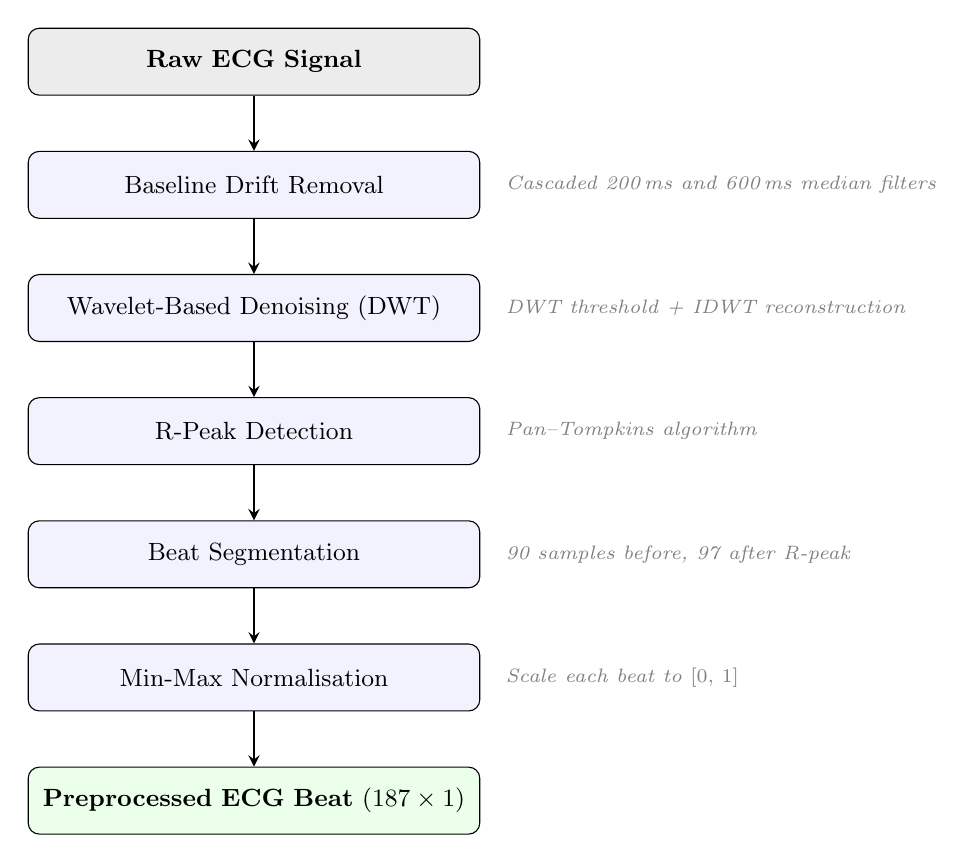
\begin{tikzpicture}[
        >=stealth,
        node distance=0.7cm,
        block/.style={draw, rectangle, rounded corners, fill=blue!5,
            text width=5.5cm, align=center, minimum height=0.85cm, font=\small},
        container/.style={draw, dashed, thick, inner sep=0.3cm,
            fill=gray!5, rounded corners},
        line/.style={draw, thick, ->},
        note/.style={font=\scriptsize\itshape, text=black!50, anchor=west},
    ]
        \node[block, fill=gray!15] (s1) {\textbf{Raw ECG Signal}};
        \node[block, below=of s1] (s2) {Baseline Drift Removal};
        \node[block, below=of s2] (s3) {Wavelet-Based Denoising (DWT)};
        \node[block, below=of s3] (s4) {R-Peak Detection};
        \node[block, below=of s4] (s5) {Beat Segmentation};
        \node[block, below=of s5] (s6) {Min-Max Normalisation};
        \node[block, fill=green!8, below=of s6] (s7)
            {\textbf{Preprocessed ECG Beat} ($187 \times 1$)};
 
        \foreach \i/\j in {s1/s2, s2/s3, s3/s4, s4/s5, s5/s6, s6/s7}
            \path[line] (\i) -- (\j);
 
        \node[note, right=0.2cm of s2] {Cascaded 200\,ms and 600\,ms median filters};
        \node[note, right=0.2cm of s3] {DWT threshold + IDWT reconstruction};
        \node[note, right=0.2cm of s4] {Pan--Tompkins algorithm};
        \node[note, right=0.2cm of s5] {90 samples before, 97 after R-peak};
        \node[note, right=0.2cm of s6] {Scale each beat to $[0,\,1]$};
    \end{tikzpicture}
    }
    \caption{ECG preprocessing pipeline from raw recording to normalized 187-sample beat windows.}
    \label{fig:preprocess}
\end{figure}
 
\subsection{Class Imbalance Strategy}
\label{sec:imbalance}
Three complementary mechanisms address the pronounced class imbalance in MIT-BIH.
 
\textbf{SMOTE oversampling.} Synthetic Minority Oversampling Technique (SMOTE) generates interpolated minority-class samples in feature space. Crucially, SMOTE is applied exclusively within the training fold, after the train/validation split, preventing any synthetic data from contaminating evaluation metrics.
 
\textbf{Inverse-frequency loss weighting.} Each training sample contributes to the loss with a weight inversely proportional to its class frequency, discouraging the optimizer from over-fitting to the majority class.
 
\textbf{Class-weighted focal loss.} The focal loss formulation used is:
\begin{equation}
    \mathcal{L}_{\text{focal}} = - \sum_{k=1}^{C} \alpha_k (1 - p_k)^{\gamma} \log(p_k)
\end{equation}
with $\gamma = 2.0$ and label smoothing $\epsilon = 0.1$. The modulating factor $(1-p_k)^\gamma$ down-weights well-classified examples, redirecting gradient signal toward hard, typically minority-class samples.
 
\subsection{CAWT Architecture}
The full architecture is shown in Fig.~\ref{fig:cawt_arch}. A 187-sample beat window is processed simultaneously by two independent branches, whose intermediate representations are repeatedly exchanged through bidirectional cross-attention before being fused for final classification.
 
\begin{figure*}[t]
    \centering
    \resizebox{\textwidth}{!}{
    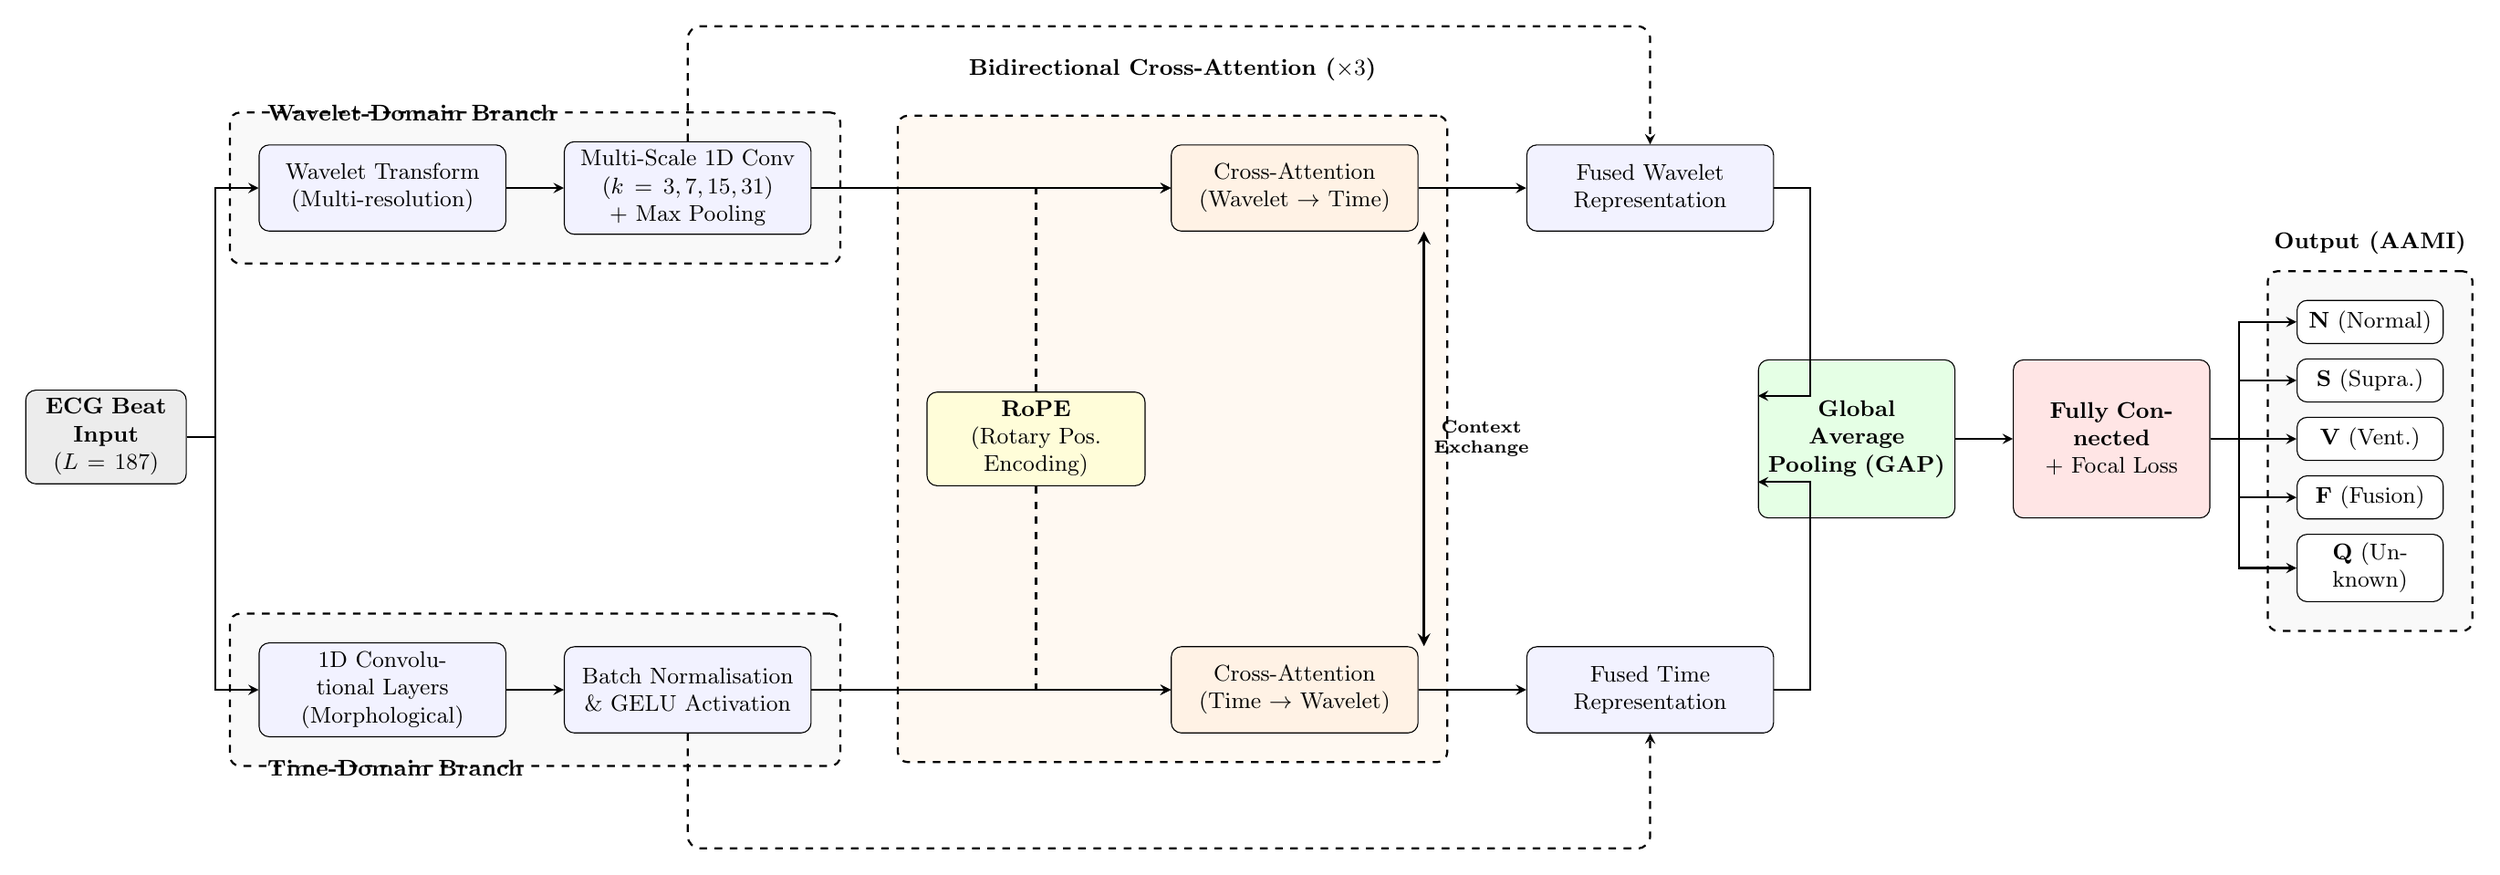
\begin{tikzpicture}[
        >=stealth,
        node distance=1.2cm and 1cm,
        block/.style={draw, rectangle, rounded corners, fill=blue!5,
            text width=3.2cm, align=center, minimum height=1.2cm, font=\small},
        wideblock/.style={block, text width=4cm, fill=gray!15},
        attnblock/.style={draw, rectangle, rounded corners, fill=orange!10,
            text width=3.2cm, align=center, minimum height=1.2cm, font=\small},
        container/.style={draw, dashed, thick, inner sep=0.4cm,
            fill=gray!5, rounded corners},
        attncontainer/.style={draw, dashed, thick, inner sep=0.4cm,
            fill=orange!5, rounded corners},
        line/.style={draw, thick, ->},
        title/.style={font=\bfseries\small},
    ]
 
    % 1. Input
    \node[block, text width=2cm, fill=gray!15] (input)
        {\textbf{ECG Beat\\Input}\\($L=187$)};
 
    % 2. Wavelet-Domain Branch (Top)
    \node[block, above right=2.2cm and 1cm of input] (wt)
        {Wavelet Transform\\(Multi-resolution)};
    \node[block, right=0.8cm of wt] (w_conv)
        {Multi-Scale 1D Conv\\($k = 3, 7, 15, 31$)\\+ Max Pooling};
    \node[title, above=0.2cm of wt.north west, anchor=south west]
        {Wavelet-Domain Branch};
 
    \begin{scope}[on background layer]
        \node[container, fit=(wt) (w_conv)] (w_box) {};
    \end{scope}
 
    % 3. Time-Domain Branch (Bottom)
    \node[block, below right=2.2cm and 1cm of input] (t_conv)
        {1D Convolutional Layers\\(Morphological)};
    \node[block, right=0.8cm of t_conv] (t_bn)
        {Batch Normalisation\\\& GELU Activation};
    \node[title, below=0.2cm of t_conv.south west, anchor=north west]
        {Time-Domain Branch};
 
    \begin{scope}[on background layer]
        \node[container, fit=(t_conv) (t_bn)] (t_box) {};
    \end{scope}
 
    % 4. Bidirectional Cross-Attention (Centre)
    \node[attnblock, right=5cm of w_conv] (w2t)
        {Cross-Attention\\(Wavelet $\rightarrow$ Time)};
    \node[attnblock, right=5cm of t_bn] (t2w)
        {Cross-Attention\\(Time $\rightarrow$ Wavelet)};
    \node[block, fill=yellow!15, text width=2.8cm, minimum height=0.8cm]
        at ($(w2t)!0.5!(t2w) + (-3.6cm, 0)$) (rope)
        {\textbf{RoPE}\\(Rotary Pos.\\Encoding)};
 
    \begin{scope}[on background layer]
        \node[attncontainer, fit=(w2t) (t2w) (rope)] (attn_box) {};
        \node[title, above=0.35cm of attn_box.north]
            {Bidirectional Cross-Attention ($\times 3$)};
    \end{scope}
 
    % 5. Feature Fusion
    \node[block, right=1.5cm of w2t] (w_fuse)
        {Fused Wavelet\\Representation};
    \node[block, right=1.5cm of t2w] (t_fuse)
        {Fused Time\\Representation};
 
    % 6. GAP and Classification
    \node[block, fill=green!10, text width=2.5cm, minimum height=2.2cm,
          right=1.5cm of $(w_fuse)!0.5!(t_fuse)$] (gap)
        {\textbf{Global Average\\Pooling (GAP)}};
    \node[block, fill=red!10, text width=2.5cm, minimum height=2.2cm,
          right=0.8cm of gap] (fc)
        {\textbf{Fully Connected}\\+ Focal Loss};
 
    % 7. Output Classes
    \node[block, fill=white, text width=1.8cm, minimum height=0.6cm,
          right=1.2cm of fc] (classV) {\textbf{V} (Vent.)};
    \node[block, fill=white, text width=1.8cm, minimum height=0.6cm,
          above=0.2cm of classV] (classS) {\textbf{S} (Supra.)};
    \node[block, fill=white, text width=1.8cm, minimum height=0.6cm,
          above=0.2cm of classS] (classN) {\textbf{N} (Normal)};
    \node[block, fill=white, text width=1.8cm, minimum height=0.6cm,
          below=0.2cm of classV] (classF) {\textbf{F} (Fusion)};
    \node[block, fill=white, text width=1.8cm, minimum height=0.6cm,
          below=0.2cm of classF] (classQ) {\textbf{Q} (Unknown)};
 
    \begin{scope}[on background layer]
        \node[container, fill=gray!5, fit=(classN) (classQ)] (out_box) {};
        \node[title, above=0.1cm of out_box.north] {Output (AAMI)};
    \end{scope}
 
    % --- Arrows ---
    \path[line] (input.east) -- ++(0.4,0) |- (wt.west);
    \path[line] (input.east) -- ++(0.4,0) |- (t_conv.west);
    \path[line] (wt) -- (w_conv);
    \path[line] (t_conv) -- (t_bn);
    \path[line] (w_conv) -- (w2t);
    \path[line] (t_bn) -- (t2w);
    \path[line, dashed] (rope.north) |- (w2t.west);
    \path[line, dashed] (rope.south) |- (t2w.west);
    \path[line, <->, very thick]
        ([xshift=1.8cm]w2t.south) -- ([xshift=1.8cm]t2w.north)
        node[midway, right, font=\scriptsize\bfseries, align=center]
        {Context\\Exchange};
    \path[line] (w2t) -- (w_fuse);
    \path[line] (t2w) -- (t_fuse);
    \path[line, dashed, rounded corners=5pt]
        (w_conv.north) -- ++(0, 1.6) -| (w_fuse.north);
    \path[line, dashed, rounded corners=5pt]
        (t_bn.south) -- ++(0,-1.6) -| (t_fuse.south);
    \path[line] (w_fuse.east) -- ++(0.5,0) |- ([yshift= 0.6cm]gap.west);
    \path[line] (t_fuse.east) -- ++(0.5,0) |- ([yshift=-0.6cm]gap.west);
    \path[line] (gap) -- (fc);
    \path[line] (fc.east) -- ++(0.4,0) |- (classN.west);
    \path[line] (fc.east) -- ++(0.4,0) |- (classS.west);
    \path[line] (fc.east) -- (classV.west);
    \path[line] (fc.east) -- ++(0.4,0) |- (classF.west);
    \path[line] (fc.east) -- ++(0.4,0) |- (classQ.west);
 
    \end{tikzpicture}
    }
    \caption{CAWT architecture. Both branches receive the same 187-sample beat and interact through three stages of bidirectional cross-attention (RoPE-guided) before their fused representations are pooled and classified.}
    \label{fig:cawt_arch}
\end{figure*}
 
\begin{figure}[ht]
    \centering
    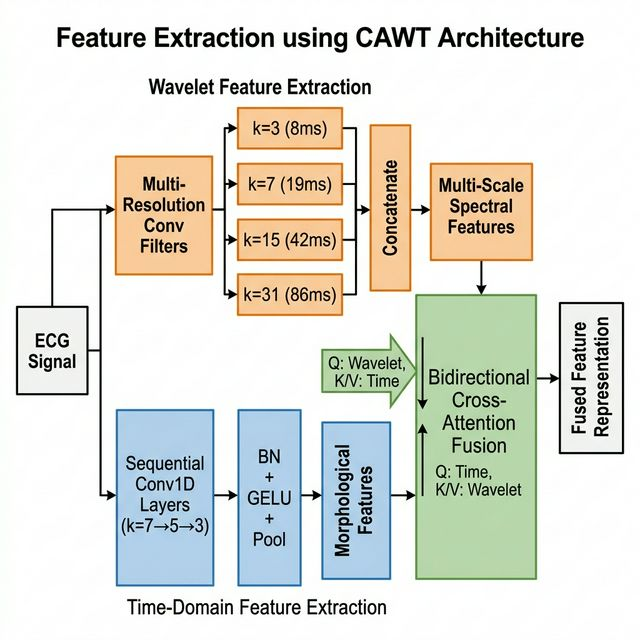
\includegraphics[width=\columnwidth]{feature_extraction.png}
    \caption{Detailed feature extraction pipeline showing the wavelet-domain branch (multi-resolution convolutional filters at 8--86~ms scales) and the time-domain branch (sequential Conv1D layers), merged through bidirectional cross-attention fusion.}
    \label{fig:feature_extract}
\end{figure}
 
\subsubsection{Multi-Scale Spectral Branch}
This branch treats the beat window as a multi-resolution signal, applying four parallel 1D convolutional filters with kernel sizes of 3, 7, 15, and 31 samples. At 360~Hz, these kernels span approximately 8~ms, 19~ms, 42~ms, and 86~ms, capturing structures ranging from the narrow QRS complex to broad P-wave and T-wave envelopes. Outputs from each kernel are concatenated along the channel dimension, passed through Batch Normalization, and activated with GELU, which preserves gradient flow through near-zero activations. The branch is initiated by a stem convolution with kernel size 7 and stride 2 that halves the temporal resolution before the parallel kernels are applied.
 
\subsubsection{Compact Temporal Branch}
The temporal branch processes the raw beat through three successive 1D convolutional layers with kernel sizes 7, 5, and 3. The first layer uses stride 2 to halve temporal resolution (matching the wavelet branch). A single MaxPool1d layer sits between the second and third convolutions to further downsample. Each convolution is followed by Batch Normalization and GELU activation.
 
\subsubsection{Bidirectional Cross-Attention with RoPE}
The core idea behind CAWT is letting the two branches talk during feature extraction, not just at the end. At each of three stages, the spectral branch queries the temporal branch (Wavelet $\to$ Time), and the temporal branch queries back (Time $\to$ Wavelet). Both branches update based on what the other has learned so far.
 
Initially, learned additive positional encodings were tried, but they interfered with the model's ability to pick up on relative timing between ECG features (for example, the PR interval or QT duration depends on sample-to-sample spacing, not absolute position). Switching to Rotary Position Embeddings (RoPE) fixed this. RoPE encodes position by rotating query and key vectors:
\begin{equation}
    \mathbf{q}_m = \mathbf{x}_m \mathbf{W}_q \mathbf{R}_{\Theta, m}
\end{equation}
where $\mathbf{R}_{\Theta,m}$ is a rotation matrix parameterized by position $m$ and frequency $\Theta$. Because only the dot product between queries and keys appears in the attention score, RoPE naturally encodes the relative gap between two positions without modifying the representations themselves. This property is well-suited to ECG analysis, where physiologically meaningful intervals (e.g., PR interval, QT duration) are defined by relative sample distances rather than absolute positions. Stochastic depth regularization (DropPath) is applied to each cross-attention block with linearly increasing drop rates from 0 to 0.15 across the three stages.
 
\subsection{Training Configuration}
Parameters are optimized with AdamW, which decouples weight decay from adaptive gradient scaling:
\begin{equation}
    \theta_{t} = \theta_{t-1} - \eta_t \left( \alpha \frac{\hat{m}_t}{\sqrt{\hat{v}_t} + \epsilon} + \lambda \theta_{t-1} \right)
\end{equation}
with weight decay $\lambda = 0.05$. The learning rate follows a OneCycleLR schedule peaking at $3 \times 10^{-4}$. Training runs for a budget of 80 epochs with early stopping (patience of 20 epochs on macro F1). Data augmentation during training includes additive Gaussian noise ($\sigma = 0.02$), synthetic baseline wander, random amplitude scaling ($[0.9, 1.1]$), and random zero-masking of 10\% of the signal. All experiments are run on an NVIDIA GPU with automatic mixed precision (FP16).
 
% ============================================================================
% IV. RESULTS
% ============================================================================
\section{Experimental Results}
 
\subsection{Baseline Comparisons}
Before evaluating the full CAWT, each branch was trained in isolation to understand what it contributes on its own. Same data, same optimizer, same augmentation; the only difference is the architecture.
 
The WaveletCNN baseline (spectral branch alone, no cross-attention) hits 89.95\% accuracy, weighted F1 of 0.88, macro F1 of 0.84. It does well on normal beats but almost completely ignores the minority classes; class S and class F recall were both near zero. This makes sense: the WaveletCNN sees local frequency patterns but has no way to reason about sequence-level context.
 
The Transformer alone does better: 95.53\% accuracy, weighted F1 of 0.95, macro F1 of 0.92. Its self-attention helps with most minority classes, but class F (fusion beats) still gave trouble. Fusion beats are part-normal, part-ventricular. Catching them requires both the fine-grained waveform shape and the broader temporal context, and a pure Transformer operating on a flat token stream struggles with that.

\begin{figure}[ht]
    \centering
    \includegraphics[width=\columnwidth]{{Wavelet Validation Accuracy and Validation MacroF1}.jpg}
    \caption{Wavelet CNN baseline: validation accuracy (left) and macro F1 (right) over 80 epochs. Peak accuracy reaches approximately 91\% but macro F1 plateaus below the 90\% target.}
    \label{fig:wavelet_val}
\end{figure}

\begin{figure}[ht]
    \centering
    \includegraphics[width=\columnwidth]{{Transformer Validation Accuracy and Validation MacroF1}.jpg}
    \caption{Transformer baseline: validation accuracy (left) and macro F1 (right) over 80 epochs. Accuracy approaches 96\% and macro F1 reaches approximately 93\%, surpassing the CNN baseline but remaining below the CAWT.}
    \label{fig:transformer_val}
\end{figure}

\begin{figure}[ht]
    \centering
    \includegraphics[width=\columnwidth]{{Accuracy comparision of Wavelwt and transformer}.jpg}
    \caption{Training accuracy comparison between WaveletCNN and Transformer baselines. The Transformer converges faster and achieves consistently higher accuracy.}
    \label{fig:baseline_acc}
\end{figure}

\begin{figure}[ht]
    \centering
    \includegraphics[width=\columnwidth]{{Normalised Confusion Matrix of Wavelet and Transformer}.jpg}
    \caption{Normalized confusion matrices for the WaveletCNN (left) and Transformer (right) baselines. The WaveletCNN completely fails on classes S and F (0\% recall each), while the Transformer partially recovers S (45\%) and F (8\%) but still performs poorly on minority classes.}
    \label{fig:baseline_cm}
\end{figure}
 
\subsection{Full CAWT Performance}
The complete CAWT model converges at epoch 79 of 80, with a typical training time of approximately 83 seconds per epoch. Overall results are summarized in Table~\ref{tab:cawt_results}.
 
\begin{table}[ht]
\centering
\caption{CAWT Overall Performance}
\label{tab:cawt_results}
\footnotesize
\begin{tabular}{@{}lc@{}}
\toprule
\textbf{Metric} & \textbf{Value} \\
\midrule
Overall Accuracy & 99.00\% \\
Weighted F1 & 0.99 \\
Macro F1 & 93.77\% \\
AUROC (macro) & 0.9883 \\
\bottomrule
\end{tabular}
\end{table}
 
\subsubsection{Per-Class Results}
Table~\ref{tab:perclass} shows classification accuracy for each AAMI class on the held-out test set. Ventricular ectopic beats (class V) are identified with 99\% recall, reflecting the pronounced QRS morphology difference from normal beats. Fusion beats (class F) achieve 88\% recall, the lowest among all classes. These beats share partial morphological characteristics with both normal and ventricular complexes, making them inherently ambiguous. The rare supraventricular class (S) reaches 96\%, demonstrating that the SMOTE and focal loss strategy is effective even at 2.54\% prevalence.
 
\begin{table}[ht]
\centering
\caption{Per-Class Recall on the Test Set (Normalized Confusion Matrix Diagonal)}
\label{tab:perclass}
\footnotesize
\begin{tabular}{@{}lc@{}}
\toprule
\textbf{Class} & \textbf{Recall} \\
\midrule
N & 99\% \\
S & 96\% \\
V & 99\% \\
F & 88\% \\
Q & 100\% \\
\bottomrule
\end{tabular}
\end{table}
 
\subsubsection{Confusion Matrix}
Fig.~\ref{fig:confusion} shows the confusion matrix on the test set. The dominant off-diagonal errors occur between class F and both class N and class V, consistent with the hybrid origin of fusion beats and with patterns reported in manual expert annotation studies~\cite{dechazal2004}.
 
\begin{figure}[ht]
    \centering
    \includegraphics[width=\columnwidth]{{CAWT Normalised Confusion Matrix}.jpg}
    \caption{Normalized confusion matrix on the test set. Rows are true labels; columns are predicted labels. Class~F (fusion) shows the most confusion, misclassified primarily as N (0.07) and V (0.04).}
    \label{fig:confusion}
\end{figure}
 
\subsubsection{ROC Analysis}
Per-class AUROC values are given in Table~\ref{tab:auc} and the corresponding ROC curves are plotted in Fig.~\ref{fig:roc}. All five classes exceed AUC 0.96, with classes N, V, and Q approaching or reaching 0.999. Class~F, while showing the lowest AUC at 0.963, still represents strong discriminative ability given the morphological overlap with neighboring classes.
 
\begin{table}[ht]
\centering
\caption{Per-Class AUROC}
\label{tab:auc}
\footnotesize
\begin{tabular}{@{}lc@{}}
\toprule
\textbf{Class} & \textbf{AUROC} \\
\midrule
N & 0.995 \\
S & 0.979 \\
V & 0.997 \\
F & 0.963 \\
Q & 0.999 \\
\bottomrule
\end{tabular}
\end{table}
 
\begin{figure}[ht]
    \centering
    \includegraphics[width=\columnwidth]{{CAWT ROC curves}.jpg}
    \caption{ROC curves (one-vs-rest) for all five AAMI classes.}
    \label{fig:roc}
\end{figure}
 
\begin{figure}[ht]
    \centering
    \includegraphics[width=\columnwidth]{{CAWT training and validation loss graph}.jpg}
    \caption{Training and validation loss curves over 80 epochs.}
    \label{fig:training_curves}
\end{figure}
 
\subsection{Model Comparison}
Table~\ref{tab:comparison} summarizes the progression from individual-branch baselines to the full integrated model. CAWT's 99.00\% accuracy represents a 9.05 percentage-point gain over the WaveletCNN baseline and a 3.47 percentage-point gain over the Transformer baseline. The macro F1 improvement from 0.84 to 0.9377 reflects gains concentrated in the three minority classes.
 
\begin{table}[H]
\centering
\caption{Architecture Comparison}
\label{tab:comparison}
\footnotesize
\begin{tabular}{@{}lcccl@{}}
\toprule
\textbf{Model} & \textbf{Accuracy} & \textbf{F1 (W)} & \textbf{F1 (M)} & \textbf{AUROC} \\
\midrule
WaveletCNN & 89.95\% & 0.88 & 0.84 & 0.90 \\
Transformer & 95.53\% & 0.95 & 0.92 & 0.96 \\
\textbf{CAWT (full)} & \textbf{99.00\%} & \textbf{0.99} & \textbf{0.9377} & \textbf{0.9883} \\
\bottomrule
\end{tabular}
\end{table}
 
\subsection{Computational Cost}
Table~\ref{tab:computational} shows that CAWT's 1.66 million parameters are 1.96$\times$ the size of the Transformer baseline and only slightly over twice the WaveletCNN baseline, yet the accuracy gain is substantial. The parameter count remains well within the range feasible for edge deployment or embedded clinical devices.
 
\begin{table}[H]
\centering
\caption{Parameter Count vs. Performance}
\label{tab:computational}
\footnotesize
\begin{tabular}{@{}lcc@{}}
\toprule
\textbf{Model} & \textbf{Parameters} & \textbf{Accuracy} \\
\midrule
WaveletCNN & $\approx$0.42 M & 89.95\% \\
Transformer & $\approx$0.85 M & 95.53\% \\
\textbf{CAWT (full)} & \textbf{1.66 M} & \textbf{99.00\%} \\
\bottomrule
\end{tabular}
\end{table}
 
\subsection{Ablation Study}
To figure out how much each design choice contributes, four variants were trained that progressively introduce the bidirectional coupling mechanism (Table~\ref{tab:ablation}). All variants share the same preprocessing, data augmentation, and loss configuration so the only thing changing is the architecture.
 
\begin{table}[H]
\centering
\caption{Ablation Results}
\label{tab:ablation}
\footnotesize
\begin{tabular}{@{}lcc@{}}
\toprule
\textbf{Configuration} & \textbf{Accuracy} & \textbf{Macro F1} \\
\midrule
Late fusion (no cross-attention) & 96.12\% & 89.45\% \\
Unidirectional cross-attention & 97.85\% & 91.32\% \\
Bidirectional, 1 stage ($N=1$) & 98.21\% & 92.10\% \\
Bidirectional, 3 stages ($N=3$) & \textbf{99.00\%} & \textbf{93.77\%} \\
\bottomrule
\end{tabular}
\end{table}
 
The ablation numbers are straightforward. Without any cross-attention (late fusion), accuracy falls to 96.12\% and macro F1 to 89.45\%. Adding one-way attention (spectral queries temporal, but not the reverse) recovers some performance, but the temporal branch is still flying blind. Bidirectional coupling at a single depth helps more. Going to three stages gives the best result. $N=5$ was also tried during development but it did not improve further, suggesting three rounds of exchange are enough for this dataset.
 
\subsection{Comparison with Published Methods}
Table~\ref{tab:sota} compares CAWT against closely related hybrid CNN-Transformer architectures evaluated on the MIT-BIH Arrhythmia Database. Only methods that combine convolutional and attention-based components and report accuracy on the same dataset are included. All values are taken directly from the respective original publications.

\begin{table}[H]
\centering
\caption{Comparison with Attention-Based Architectures on MIT-BIH}
\label{tab:sota}
\footnotesize
\begin{tabular}{@{}llc@{}}
\toprule
\textbf{Method} & \textbf{Type} & \textbf{Accuracy} \\
\midrule
He et al.~\cite{he2025} & BiLSTM + Attention & 94.41\% \\
Saadatnejad et al.~\cite{saadatnejad2020} & Wavelet + LSTM & 97.40\% \\
\midrule
\textbf{CAWT (ours)} & \textbf{Dual-branch + RoPE} & \textbf{99.00\%} \\
\bottomrule
\end{tabular}
\end{table}

Among hybrid attention-based architectures on the MIT-BIH database, CAWT posts the highest accuracy at 99.00\%. Saadatnejad et al.~\cite{saadatnejad2020} combine wavelet features with LSTM networks for wearable deployment, reaching 97.40\%, but there is no cross-attention mechanism between their feature branches. He et al.~\cite{he2025} pair BiLSTM with multi-head attention and report 94.41\% averaged across external test sets. CAWT beats both by 1.60 and 4.59 percentage points respectively, and the ablation numbers suggest most of that gain comes from the bidirectional coupling across three successive depths.

% ============================================================================
% V. MOBILE APPLICATION DEPLOYMENT
% ============================================================================
\section{Mobile Application Deployment}

To demonstrate the practical applicability of the trained CAWT model, an Android application named \textbf{CardioScan} was developed. The application provides a user-friendly interface for real-time ECG beat classification on commodity smartphones, serving as a proof-of-concept for point-of-care arrhythmia screening.

\subsection{Application Architecture}
The trained CAWT model was exported from PyTorch to TorchScript Lite format, enabling efficient on-device inference without requiring a network connection. The application was built using Kotlin in Android Studio and supports three input modes:

\begin{enumerate}
    \item \textbf{Manual entry:} The user pastes 187 comma-separated amplitude values directly into a text field.
    \item \textbf{CSV import:} A pre-recorded ECG beat file is loaded from device storage.
    \item \textbf{Demo mode:} Built-in sample beats for each AAMI class allow immediate testing without external data.
\end{enumerate}

Upon classification, the app displays the predicted AAMI class label, a confidence score, a color-coded donut chart showing class probability distribution, and the rendered ECG waveform. Fig.~\ref{fig:app_interface} shows the main interface of the application.

\begin{figure}[ht]
    \centering
    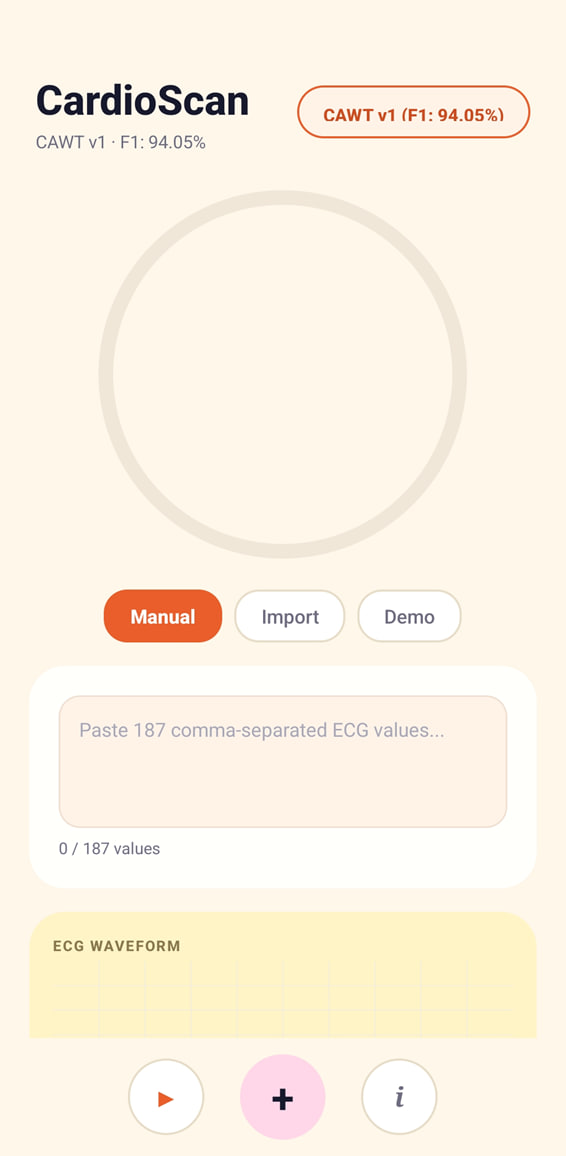
\includegraphics[width=0.55\columnwidth]{app_interface.jpg}
    \caption{CardioScan main interface showing the input modes (Manual, Import, Demo), ECG waveform display, and the classification ring indicator.}
    \label{fig:app_interface}
\end{figure}

\subsection{Classification Demonstrations}
To illustrate the on-device inference pipeline, two representative cases are examined: a Normal beat (class~N) and a Fusion beat (class~F). These two classes were chosen because they represent the easiest and hardest classification scenarios respectively, as established in the confusion matrix analysis (Section~IV-B).

\textbf{Normal beat classification.} Fig.~\ref{fig:apk_normal_ring} shows the classification ring for a Normal sinus rhythm beat. The donut chart is dominated by green, and the app assigns the correct label with a top-class probability of 67\%. The full probability breakdown (Fig.~\ref{fig:apk_normal_prob}) shows that the remaining probability mass is distributed nearly uniformly across the other four classes (S: 8\%, V: 7\%, F: 8\%, Q: 8\%), indicating that the model is confident in its prediction with no competing hypothesis. The rendered ECG waveform displays a clean QRS complex with a well-defined R-peak, consistent with normal sinus morphology.

\begin{figure}[H]
    \centering
    \begin{minipage}{0.48\columnwidth}\centering
        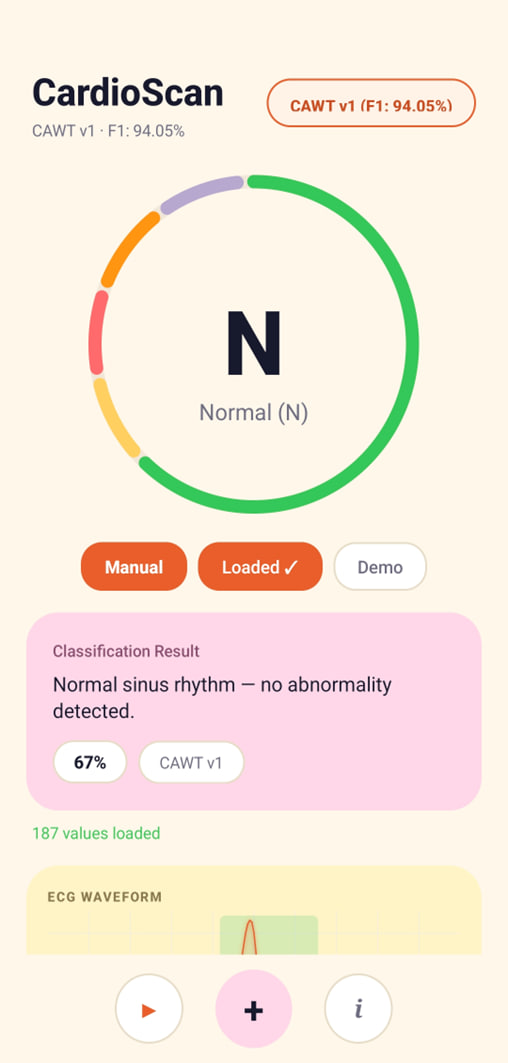
\includegraphics[width=0.85\textwidth]{normal_screenshot_1.jpg}
    \end{minipage}\hfill
    \begin{minipage}{0.48\columnwidth}\centering
        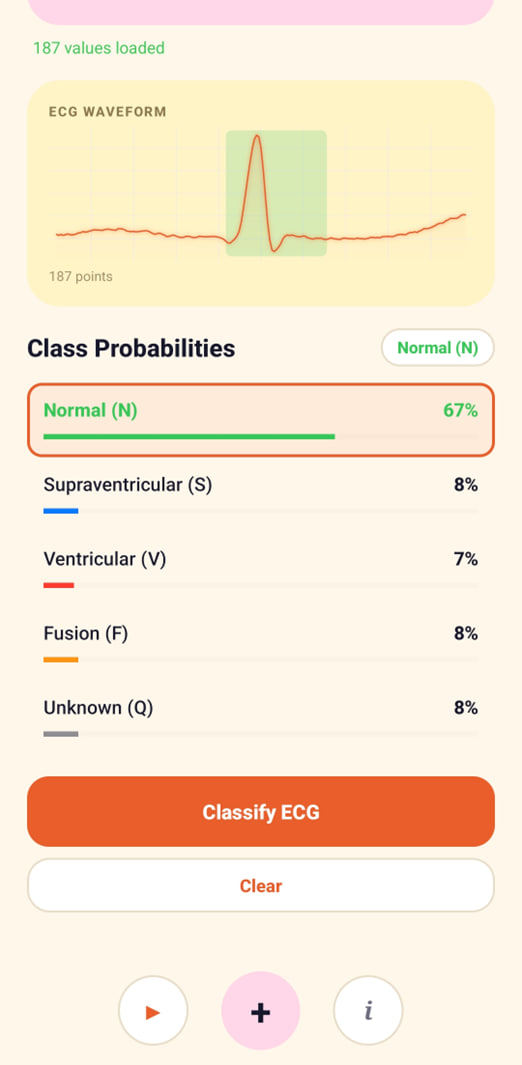
\includegraphics[width=0.85\textwidth]{normal_screenshot_2.jpg}
    \end{minipage}
    \caption{Normal beat: (left) classification ring showing dominant N prediction, (right) class probability distribution with 67\% confidence for Normal.}
    \label{fig:apk_normal_ring}
    \label{fig:apk_normal_prob}
\end{figure}

\textbf{Fusion beat classification.} Fig.~\ref{fig:apk_fusion_ring} shows the classification output for a Fusion beat. Fusion beats are inherently ambiguous because they arise from the simultaneous activation of a normal sinus impulse and a ventricular ectopic focus, producing a waveform that blends characteristics of both. The model correctly identifies the beat as class~F with 65\% confidence. The probability breakdown (Fig.~\ref{fig:apk_fusion_prob}) reveals that Ventricular (V) receives the second-highest probability at 11\%, reflecting the morphological overlap between fusion and ventricular complexes. This leakage pattern is consistent with the off-diagonal errors observed in the confusion matrix (Fig.~\ref{fig:confusion}), where class~F is most frequently misclassified as N (7\%) and V (4\%). The remaining classes (N: 7\%, S: 7\%, Q: 7\%) share the residual probability mass roughly equally.

\begin{figure}[H]
    \centering
    \begin{minipage}{0.48\columnwidth}\centering
        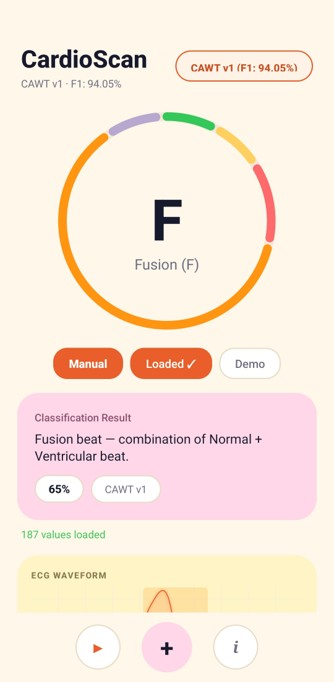
\includegraphics[width=0.85\textwidth]{fusion_screenshot_1.jpg}
    \end{minipage}\hfill
    \begin{minipage}{0.48\columnwidth}\centering
        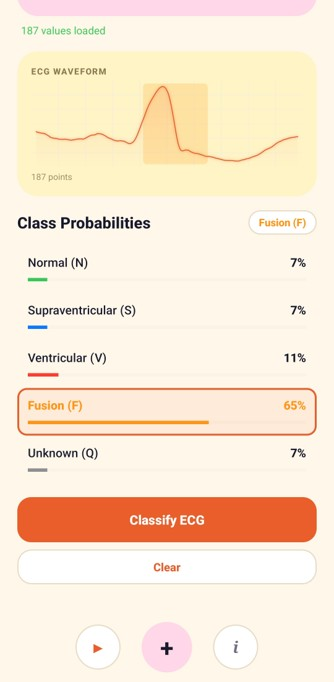
\includegraphics[width=0.85\textwidth]{fusion_screenshot_2.jpg}
    \end{minipage}
    \caption{Fusion beat: (left) classification ring showing F prediction, (right) class probability distribution with 65\% confidence and 11\% leakage to Ventricular.}
    \label{fig:apk_fusion_ring}
    \label{fig:apk_fusion_prob}
\end{figure}

The contrast between these two cases highlights an important property of the deployed model: even for the most challenging class in the dataset, the on-device inference produces a correct prediction with interpretable confidence scores. The remaining three classes---Supraventricular~(S), Ventricular~(V), and Unknown~(Q)---were also tested using their respective sample beats and were correctly identified by the application in each case, consistent with the per-class recall figures reported in Table~\ref{tab:perclass}. The 1.66~M parameter CAWT model runs with sub-second inference latency on commodity smartphone hardware, validating the feasibility of deploying the model in resource-constrained clinical and ambulatory settings.

% ============================================================================
% VI. CONCLUSION
% ============================================================================
\section{Conclusion}
 
This paper presented CAWT, which pairs a multi-scale WaveletCNN branch with a temporal Transformer branch and has them exchange context at three intermediate depths through bidirectional cross-attention under RoPE. On the MIT-BIH five-class benchmark the model reaches 99.00\% accuracy, 93.77\% macro F1, and 0.9883 AUROC. The ablation study made it clear that the bidirectional coupling is the single biggest contributor: stripping it out and falling back to late fusion drops accuracy to 96.12\%. On the class-imbalance side, the combination of post-split SMOTE, inverse-frequency weighting, and focal loss raised fusion-beat (class F) recall from 0\% in the WaveletCNN baseline to 88\%, for a class that makes up less than 1\% of the dataset.
 
There are obvious next steps. So far CAWT has only been tested on MIT-BIH; running it on PTB-XL or CPSC-2018 would show whether the architecture generalizes or just memorizes this particular dataset's patterns. The model sits at 1.66~M parameters, which is small by current standards but still too large for a low-power wearable, so pruning and quantization are worth trying. Also, CAWT currently sees only a single lead. Extending the bidirectional coupling to multi-lead inputs could capture spatial information that single-lead analysis misses entirely.
 
% ============================================================================
% REFERENCES
% ============================================================================
\begin{thebibliography}{99}
 
\bibitem{lee2024}
C.-C.~Lee, C.-C.~Chuang, C.-H.~Yeng, E.-C.~So, and Y.-J.~Chen, ``A cross-stage partial network and a cross-attention-based Transformer for an electrocardiogram-based cardiovascular disease decision system,'' \emph{Bioengineering}, vol.~11, no.~6, Art.~no.~564, 2024.
 
\bibitem{he2025}
Y.~He \emph{et al.}, ``CardioAttentionNet: Advancing ECG beat characterization with a high-accuracy and portable deep learning model,'' \emph{Frontiers Cardiovasc. Med.}, vol.~12, Art.~no.~1473482, 2025.
 
\bibitem{ullah2024}
M.~Ullah \emph{et al.}, ``Machine learning-based cardiovascular disease detection using optimal feature selection,'' \emph{IEEE Access}, vol.~12, pp.~16431--16446, 2024.
 
\bibitem{philip2023}
A.~M.~Philip and S.~Hemalatha, ``A performance analysis of advanced machine learning techniques for arrhythmia detection,'' in \emph{Proc. IEEE Int. Conf. Metaverse Comput. Netw. Commun. (MetaCom)}, pp.~623--629, 2023.
 
\bibitem{saadatnejad2020}
S.~Saadatnejad, M.~Oveisi, and M.~Hashemi, ``LSTM-based ECG classification for continuous monitoring on personal wearable devices,'' \emph{IEEE J. Biomed. Health Inform.}, vol.~24, no.~2, pp.~515--523, Feb.~2020.
 
\bibitem{cai2020}
J.~Cai, W.~Sun, J.~Guan, and I.~You, ``Multi-ECGNet for ECG arrhythmia multi-label classification,'' \emph{IEEE Access}, vol.~8, pp.~110848--110858, 2020.
 
\bibitem{wei2025}
L.~Wei and Y.~Li, ``A multi-scale CNN--Transformer parallel network for 12-lead ECG signal classification,'' \emph{Signal Image Video Process.}, vol.~19, no.~8, Art.~no.~611, 2025.
 
\bibitem{hu2022}
R.~Hu, J.~Chen, and L.~Zhou, ``A transformer-based deep neural network for arrhythmia detection using continuous ECG signals,'' \emph{Comput. Biol. Med.}, vol.~144, Art.~no.~105325, 2022.
 
\bibitem{kim2025}
D.~Kim, K.~R.~Lee, D.~S.~Lim, and C.-B.~Sohn, ``A novel hybrid CNN--Transformer model for arrhythmia detection without R-peak identification using Stockwell transform,'' \emph{Sci. Rep.}, vol.~15, Art.~no.~7817, 2025.
 
\bibitem{moody2001}
G.~B.~Moody and R.~G.~Mark, ``The impact of the MIT-BIH arrhythmia database,'' \emph{IEEE Eng. Med. Biol. Mag.}, vol.~20, no.~3, pp.~45--50, May/Jun.~2001.
 
\bibitem{goldberger2000}
A.~L.~Goldberger \emph{et al.}, ``PhysioBank, PhysioToolkit, and PhysioNet: Components of a new research resource for complex physiologic signals,'' \emph{Circulation}, vol.~101, no.~23, pp.~e215--e220, Jun.~2000.
 
\bibitem{dechazal2004}
P.~de~Chazal, M.~O'Dwyer, and R.~B.~Reilly, ``Automatic classification of heartbeats using ECG morphology and heartbeat interval features,'' \emph{IEEE Trans. Biomed. Eng.}, vol.~51, no.~7, pp.~1196--1206, Jul.~2004.
 
\bibitem{kreatsoulas2010}
C.~Kreatsoulas and S.~S.~Anand, ``The impact of social determinants on cardiovascular disease,'' \emph{Can. J. Cardiol.}, vol.~26, Suppl.~C, pp.~8C--13C, 2010.
 
\bibitem{joshi2008}
R.~Joshi, S.~Jan, Y.~Wu, and S.~MacMahon, ``Global inequalities in access to cardiovascular health care,'' \emph{J. Amer. College Cardiol.}, vol.~52, no.~23, pp.~1817--1825, 2008.
 
\bibitem{vaswani2017}
A.~Vaswani \emph{et al.}, ``Attention is all you need,'' in \emph{Advances in Neural Information Processing Systems (NeurIPS)}, vol.~30, pp.~5998--6008, 2017.
 
\bibitem{pantompkins1985}
J.~Pan and W.~J.~Tompkins, ``A real-time QRS detection algorithm,'' \emph{IEEE Trans. Biomed. Eng.}, vol.~BME-32, no.~3, pp.~230--236, Mar.~1985.
 
\bibitem{singh2022}
P.~Singh and A.~Sharma, ``Interpretation and classification of arrhythmia using deep convolutional network,'' \emph{IEEE Trans. Instrum. Meas.}, vol.~71, pp.~1--12, 2022.
 
\bibitem{abdelminaam2022}
D.~S.~AbdElminaam \emph{et al.}, ``DeepECG: Building an efficient framework for automatic arrhythmia classification,'' in \emph{Proc. IEEE MIUCC}, pp.~203--209, 2022.
 
\bibitem{dhara2025}
S.~K.~Dhara, N.~Bhanja, K.~V.~M.~Mohan, and M.~Tiwari, ``Hybrid deep learning framework for enhanced cardiovascular disease detection using ECG signal,'' \emph{South Eastern European J. Public Health}, vol.~XXVI, Suppl.~1, 2025.
 
\end{thebibliography}
 
\end{document}
